% %%%%%%%%%%%%%%%%%%%%%%%%%%%%%%%%%%%%%%%%%%%%%%%%%%%%%%%%%%%%%%%%%%%%%%%%%%%%%
% %%%%%%%%%%%%%%%%%%%%%%%%%%%%%%%%%%%%%%%% Survey of the Near-Earth Environment
% %%%%%%%%%%%%%%%%%%%%%%%%%%%%%%%%%%%%%%%%%%%%%%%%%%%%%%%%%%%%%%%%%%%%%%%%%%%%%

\chapter{The Near-Earth Environment}
  \label{ch_intro}

The 1850s were a pivotal time in human history. The United States spiraled toward the American Civil War, which would abolish slavery and consolidate the power of the federal government. A slew of conflicts in Southern Europe, such as the Austro-Sardinian War, led to the unification of modern Italy. China was beset by Western powers in the Second Opium War, while simultaneously fighting the Taiping Civil War, one of the bloodiest conflicts in human history. Origin of Species was published, the first transatlantic telegraph cable was laid, and modern epidemiology was developed in response to a Cholera outbreak in London. 

Ambivalent to these events, the Sun belched out a large CME\footnote{CME stands for Coronal Mass Ejection, an intense burst of particles and magnetic energy from the Sun.} aimed directly at Earth. The resulting geomagnetic storm\footnote{The Solar Storm of 1859 is also called the Carrington Event, after English astronomer Richard Carrington, who drew a connection between the storm's geomagnetic activity and the sunspots he had observed the day before.} caused telegraph systems to fail across the Western hemisphere\cite{green_2006}, and even electrocuted operators. Displays of the northern lights were visible as far south as Cuba. 

A CME of similar size narrowly missed Earth in 2012\cite{nasa_2012}. Had it not, it's estimated\cite{lloyds_2013} that it would have caused widespread, long-term electrical outages, with a damage toll on the order of \num{e9} dollars. 

\todo{The storm of 1859 presented compelling evidence that the Sun drives geomagnetic activity. In the decades that followed, a model took shape to describe the mechanisms of energy transfer between the Sun and the Earth. Based on auroral observations and data from ground-based magnetometers, Birkeland argued for the existence of a constant outflow of electrons and ions from the Sun -- the solar wind. The advent of high-frequency radio communication allowed Kennelly, Heaviside, and others to probe the electrical properties of the upper atmosphere. }

\todo{The study of space weather was revolutionized by the development of sounding rockets and satellites in the mid twentieth century. This allowed direct observation of the structure of the near-Earth environment, including, crucially, the waves that carry energy through it. }

\todo{Not least among these advances was the discovery of \Alfven waves. {\Alfven}ic aurora. Carry energy and particles. }

The study of space weather revolves around the transfer of energy from the Sun to the Earth. Ultra low frequency waves in particular are an important energy transport mechanism between the magnetosphere's outer boundary (at the solar wind) and its inner boundary (at the top of the atmosphere). 

% =============================================================================
% =============================================================================
% =============================================================================
\section{Steady State}


\todo{Sketch out the goneral structure of the magnetosphere, from the ionospheric current sheet (is this too generous?) to the magnetopause (a real current sheet). Talk about where gravity dominates, where field line curvature becomes apparent, and where the moon sits in all this. }

One hundred kilometers above Earth's surface, more or less, the neutral atmosphere transitions sharply into the conducting ionosphere.

From \cite{paschmann_2003}: ``In the thermosphere, the solar ultraviolet (UV) light and energetic particles precipitating from the magnetosphere produce ionization increasing with altitude. At the same time the particle density is low enough to make the recombination times of the ionized atoms and molecules sufficiently long to allow a significant fraction of the gas to remain ionized. This produces a conducting layer of the atmosphere known as the ionosphere. The ionosphere begins at $\sim\SI{65}{\km}$, has a peak plasma density between 200 and 300 km, and eventually merges with magnetospheric regions $\sim$1000--2000 km altitudes.''

The ionospheric E region is collisionally coupled to the neutrals. This decouples the ion and electron drifts, allowing currents to flow perpendicular to the magnetic field. 

\todo{\Alfven waves couple the magnetosphere to the ionosphere\cite{paschmann_2003}. Waves travel down the field line, accelerating particles to match the magnetospheric driver (for example, increased flow velocity as a result of enhanced reconnection). Bounces off of the ionosphere. May also bounce off the driver. Builds up drag and brings about equilibrium. }

\todo{Definition of a substorm comes from \cite{akasofu_1964}. \cite{mcpherron_1973} added the growth phase (previously it was just expansion and recovery). }

300

1000

3000

10,000 (2RE geocentric)

30,000 (5 RE)

Moon is at 60 RE or so. 

Tail goes back to about 100 RE. 

Ionosphere is dense enough to be shaped by gravity, but as altitude increases, magnetic field dominates.

The nitrogen density (w at sea level) drops from x at 100km to y at 1000km to z at 10**4 km.

By 10**4 km, the curvature of Earth's dipole magnetic field becomes apparent... and, between the increasing ion abundance and the decreasing strength of gravity, it dominates particle behavior.

At 10**5 km, the bow shock. On the dayside, at least. Balance between Earth's magnetic field and that of the sun. Another current sheet... This one far more intense.

Still less than halfway to the moon. That's 3e5 km.

This all takes place well within the orbit of the moon. Moon is about 60 RE away

Where are satellites? Geosynthronous? 

This with is concerned with the behavior of electromagnetic waves that propagate inside the magnetosheath, but outside the ionosphere; in fact, they play a significant role in the transport of energy from the former to the latter. 

Free electron density...

Still mostly neutrals, but collisions are so rare that they don't matter. At x, the mean free path of a neutral atom is comparable to... 

%There are a lot of interrelated things going on, so it's hard to describe Earth's environment one step at a time. Look at Scott's thesis -- he did this well, right? 

%Heliosphere, Magnetosphere, Ionosphere, Atmosphere?

%Current systems, convective systems, density profiles? 

%\begin{figure}
%  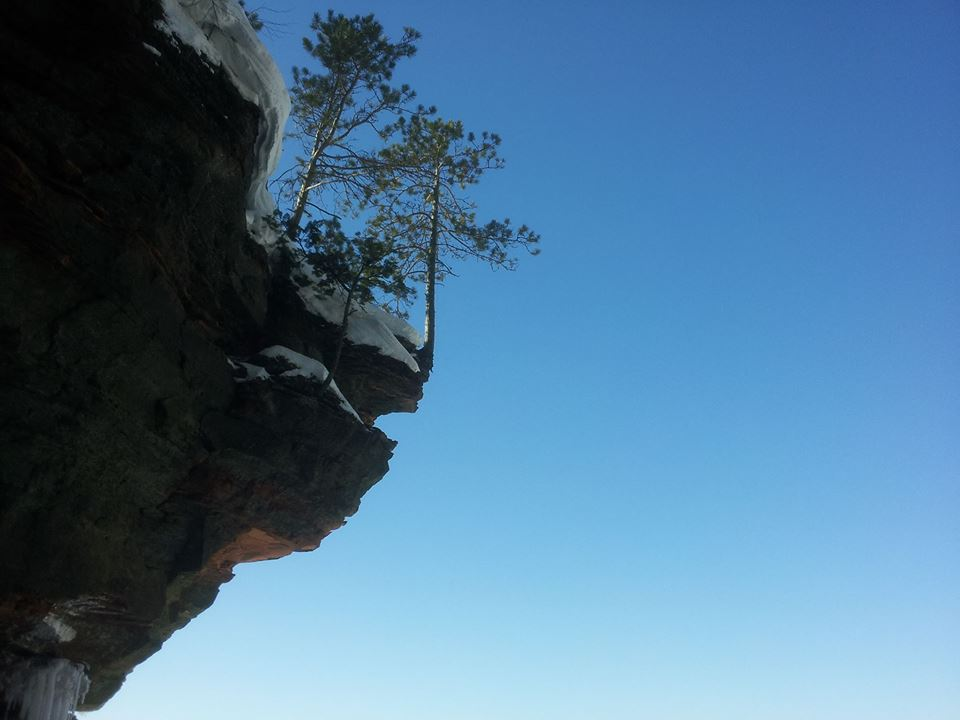
\includegraphics[width=5.75in, height=2in]{figures/image.jpg}
%  \caption{Lorem ipsum dolor sit amet, consectetur adipiscing elit, sed do eiusmod tempor incididunt ut labore et dolore magna aliqua.}
%  \label{fig_test}
%\end{figure}

It's all about energy transfer! Sun generates energy through nuclear reactions. Some of this energy is transported in the solar wind, which drives behavior in the near-Earth environment. 

%Typical solar wind density is $\sim$ \SI{5}{/\cm\cubed}. Typical solar wind velocity at Earth is \SIrange{e2}{e3}{\km/\s}. Typical solar wind particle energy is \SIrange{1}{10}{\kilo\eV}. Density can vary by $\sim$3 orders of magnitude, and velocity by one, during times of high solar activity. CMEs can also mess with the north/south component of the interplanetary magnetic field. 

At Earth's orbit, the solar magnetic field makes more-or-less a \SI{45}{\degree} angle with the \X axis. 
\footnote{Uppercase \X, \Y, and \Z are used to indicate GSE coordinates: \X points from the Earth to the Sun; \Y is perpendicular to \X in the Sun's ecliptic plane, pointing duskwards; \Z points north, out of the ecliptic plane. In later chapters, lowercase \x, \y, and \z are used to define a more-or-less analogous corodinate system with respect to Earth. }

% Solar wind is what deforms Earth's magnetic field to form the magnetosphere. 

% Transient solar wind phenomena, such as coronal mass ejections, are also known to be related to geomagnetic disturbances at Earth. Jesse cites here: 

% R. L. McPherron. Physical processes producing magnetospheric substorms and mangetic storms. In J. A. Jacobs, editor, Geomagnetism, volume 4, chapter 7. Academic Press, 1991.

% G. Rostoker. Substorms. In Handbook of the Solar-Terrestrial Environment, chapter 15. Springer-Verlag, 2007.

% This might just be worth tracking down... Jesse cites several chapters: 

% M. Shulz. Magnetospheres. In Handbook of the Solar-Terrestrial Environment, chapter 7. Springer-Verlag, 2007.

% papers mentioned during Yan's talk. mostly about alfven acceleration and nonlinear effects. 
% Vasyliunas 1970, 1984
% Hasegawa 1976
% Goertz 1991
% Stasiewicz et al 2000
% Haerendel 2008
% Song & Lysak 1994, 1999, 2000, 2001, 2006, 2011, 2012
% Inverted V?
% Double layers? 
% Charge holes? 

% -----------------------------------------------------------------------------
% -----------------------------------------------------------------------------
% -----------------------------------------------------------------------------
\subsection{The Outer Magnetosphere}


Significant deformation by the solar wind. 

Bow shock. 

Magnetopause. Current sheet consistent with \amplaw. 

Plasma sheet and PSBL. 

Tail and tail lobes. 

Reconnection. 


% -----------------------------------------------------------------------------
% -----------------------------------------------------------------------------
% -----------------------------------------------------------------------------
\subsection{The Inner Magnetosphere}

Closed field lines. More or less dipolar. 

The plasmasphere and plasmapause. 

Radiation belts. Radial diffusion is interesting because... 

\Alfven speed. So we probably want to at least mention field line resonance here? Or do we get into that in the next chapter? Plot of \Alfven speeds and \Alfven bounce times for each profile. 


% -----------------------------------------------------------------------------
% -----------------------------------------------------------------------------
% -----------------------------------------------------------------------------
\subsection{The Ionosphere}
  \label{sec_ionos}

Pedersen, Hall, and field-aligned conductivity. Do we want to get into two-cell convection? Region 1 and 2 current? 

\todo{Convection electric field. How close to Earth does it get? Don't we lose $\vec{E}=\cross{V}{B}$ when there are currents? }

``Increasing the Hall conductance allows the energy to oscillate through the inductive process rather than dissipate as Joule heating, increasing the `ringtime' of field line resonances.''\cite{waters_2013}

Scale heights. Ion/neutral composition. 

E, F layers. 

Ionospheric \Alfven resonator. This is important if we want to talk briefly about all kinds of ULF waves. 

Precipitation. Inverted V. 

\todo{Scott's thesis has a TON of detail. How much does Jesse show? }

\begin{figure}[H]
    \centering
    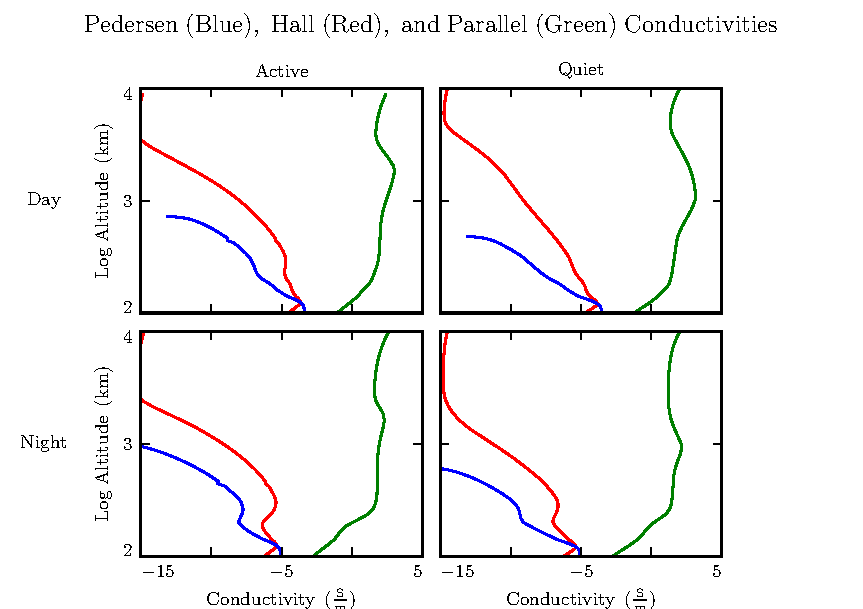
\includegraphics[width=\textwidth]{figures/sigma.pdf}
    \caption[Ionospheric Conductivity Profiles]{
      Ionospheric conductivity profiles, adapted by Lysak\cite{lysak_2013} from Appendix B of Kelley's textbook\cite{kelley_1989}. 
    }
    \label{fig_sigma}
\end{figure}


\begin{longtable}{ @{\extracolsep{\fill}} lrrr @{\extracolsep{\fill}} }
  \caption[Integrated Atmospheric Conductivity]{Integrated Atmospheric Conductivity (\si{\S})}
  \label{tab_sigma_atm} \\

  \toprule
  &
  $\Sigma_0$ &
  $\Sigma_P$ &
  $\Sigma_H$ \\
  \midrule
  \endfirsthead

  % Footer for the end of the table
  \bottomrule
  \endlastfoot

  Active Day &
  424 &
  0.65 &
  6.03 \\

  Quiet Day &
  284 &
  0.44 &
  4.02 \\

  Active Night &
  9 &
  0.01 &
  0.12 \\

  Quiet Night &
  9 &
  0.01 &
  0.12 \\

\end{longtable}

\begin{longtable}{ @{\extracolsep{\fill}} lrrr @{\extracolsep{\fill}} }
  \caption[Integrated Ionospheric Conductivity]{Integrated Ionospheric Conductivity (\si{\S})}
  \label{tab_sigma_ionos} \\

  \toprule
  &
  $\Sigma_0$ &
  $\Sigma_P$ &
  $\Sigma_H$ \\
  \midrule
  \endfirsthead

  % Footer for the end of the table
  \bottomrule
  \endlastfoot

  Active Day &
  --- &
  13.0 &
  17.0 \\

  Quiet Day &
  --- &
  5.6 &
  10.2 \\

  Active Night &
  --- &
  0.8 &
  0.3 \\

  Quiet Night &
  --- &
  0.2 &
  0.3 \\

\end{longtable}

% =============================================================================
% =============================================================================
% =============================================================================
\section{Geomagnetic Disturbances}

% -----------------------------------------------------------------------------
% -----------------------------------------------------------------------------
% -----------------------------------------------------------------------------
\subsection{Storms}

% -----------------------------------------------------------------------------
% -----------------------------------------------------------------------------
% -----------------------------------------------------------------------------
\subsection{Substorms}





Storms! CMEs, etc. 

What causes a storm. 

Storm effects: outer magnetosphere, inner magnetosphere, on the ground.






The ionospheric profiles used in this model are based on values tabulated in the Appendix B of Kelley's book\cite{kelley_1989}. They were adapted by Lysak\cite{lysak_2013} to take into account the effect of the magnetosphere's latitude-dependent density profile. 

Mean molecular mass of \SI{28}{\amu} at \SI{100}{\km}, \SI{16}{\amu} around \SI{400}{\km}, down to \SI{1}{\amu} above \SI{1400}{\km}. 

Simulations are carried out using four profiles: active day, quiet day, active night, quiet night. 

Profiles are static for the duration of a simulation. Even so-called ultra low frequency waves are still much faster than convective timescales. 

\todo{Come up with a characteristic convective timescale or two, and cite it. }

The effects of mean molecular mass on conductivity are computed per the usual definitions. 
\begin{align}
  \sp &= \displaystyle\sum_s \frac{n_s q_s^2}{m_s} \frac{\nu_s}{\nu_s^2 + \Omega_s^2} &
  \sh &= -\displaystyle\sum_s \frac{n_s q_s^2}{m_s} \frac{\Omega_s}{\nu_s^2 + \Omega_s^2} &
  \sz &= \displaystyle\sum_s \frac{n_s q_s^2}{m_s \nu_s}
\end{align}

Each profile is resolved to an altitude of about $\SI{e4}{\km}$, and include well-resolved $E$, $F_1$, and $F_2$ layers. 











